\begin{figure}[t]
    \centering
    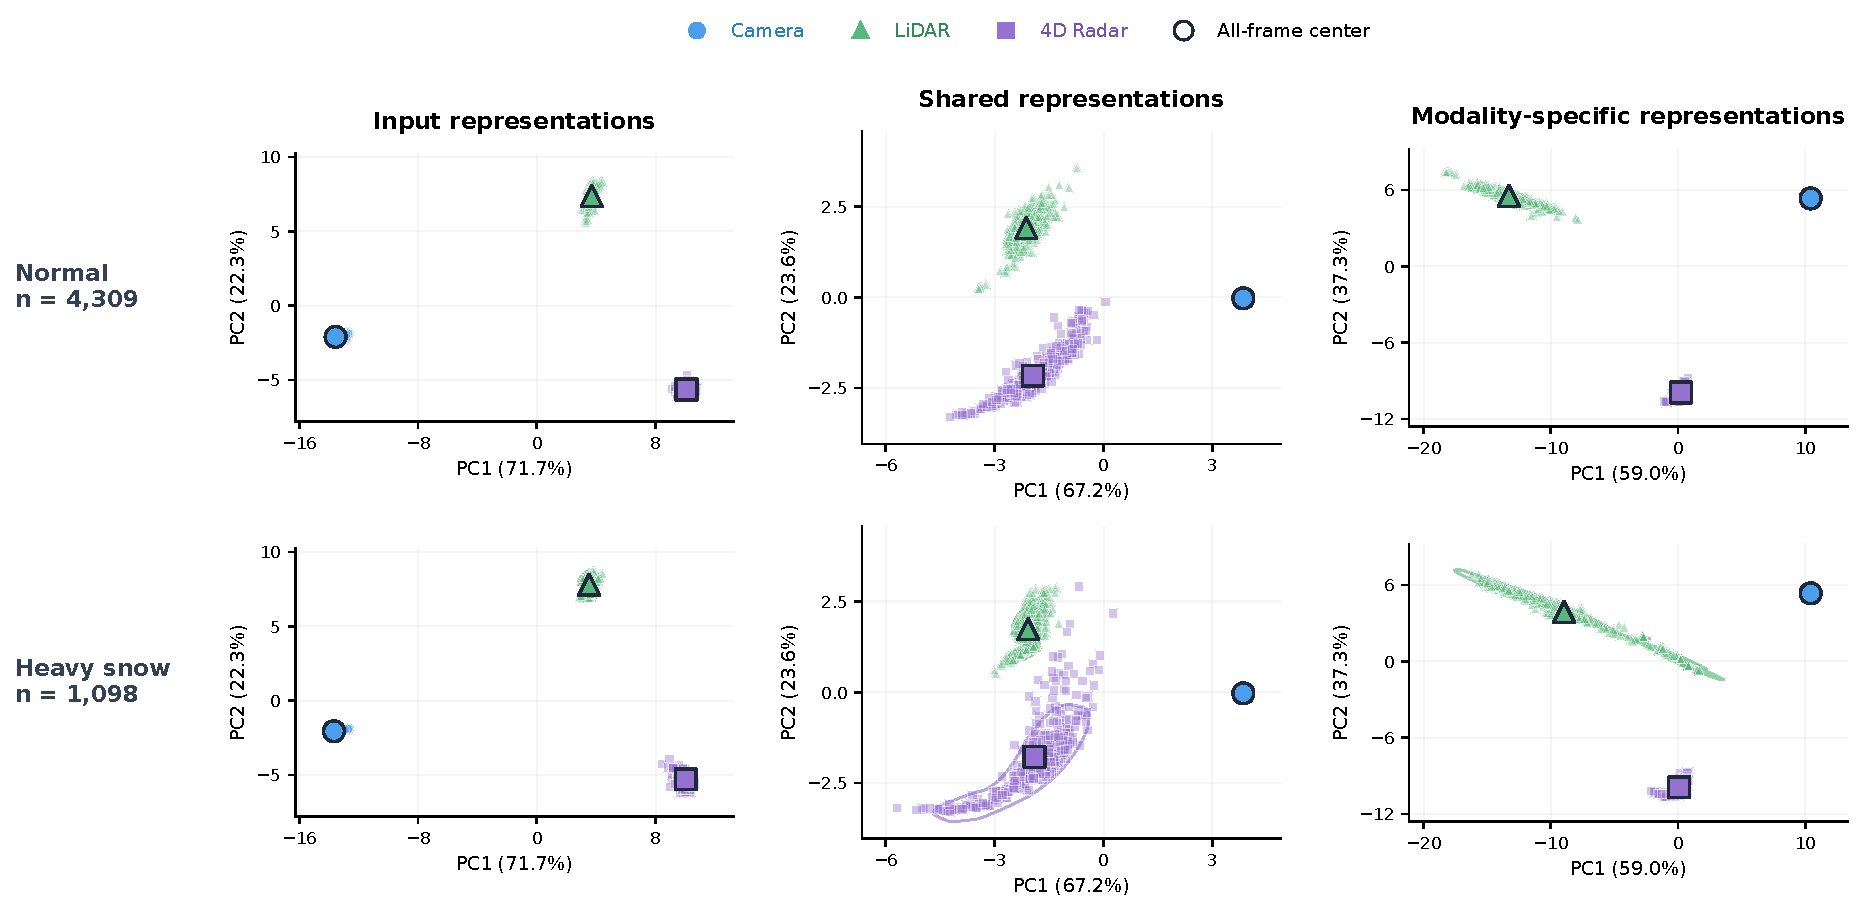
\includegraphics[width=\linewidth]{assets/figure3.pdf}
    \caption{PCA visualization of input, shared, and modality-specific representations on K-Radar v1 under normal and heavy-snow conditions. Each small marker represents the 256-dimensional feature vector averaged over all GT-defined foreground patches of one frame and one modality, projected onto two principal components. Blue circles, green triangles, and purple squares denote camera, LiDAR, and 4D radar, respectively. We display the same 400 randomly sampled frames per weather condition across all columns and modalities. Large outlined markers and density contours are computed using all frames of the corresponding weather group ($n=4{,}309$ and $1{,}098$); contours enclose approximately 80\% of the estimated density where estimation is non-degenerate. A separate PCA basis is fitted for each representation using the full test set with equal total weights for weather groups and modalities; both weather rows share that basis and axis limits within each column. Axis percentages indicate explained variance. GT is used only to select regions for this analysis.}
    \label{fig:3}
\end{figure}
